\chapter{$($TaSe$_4)_2$I, a CDW Weyl seimetal}

In Chapter \ref{ch1}, we discussed the topological phases within gapped system which exhibit gapless boundary states in lower dimension. The indispensability of maintaining an open gap underpins the nature of topological phases.  Naturally, the question arises: can we extrapolate the notion of topological phases to encompass gapless bulks? It turns out that the classification methodologies can indeed be broadened to include nodal systems featuring topological Fermi surfaces protected by symmetries\cite{matsuura2013protected, chiu2014classification, armitage2018weyl, belopolski2019discovery,fang2016topological}. The classification now depends on the codimension $p$ of such Fermi surfaces:
\begin{equation}
    p=d-d_{FS}
\end{equation}
where $d$ denotes the bulk dimension and $d_{FS}$ represents the dimension of Fermi surface inside the bulk. The Fermi surfaces can manifest in the form of nodel points, nodel lines or even nodal links\cite{yan2017nodal}. In this chapter, our attention centers on Weyl (and Dirac) semimetals, which exemplify the nodal topological phases within a three-dimensional context.

The research presented in this thesis was inspired by the recent discovery of a Weyl semimetal, $($TaSe$_4)_2$I, and its temperature-driven phase transition from a Weyl semimetal to a charge density wave. This chapter will review both the historical and recent experimental progress made with this material, in addition to exploring debates regarding its potential hosting of an intriguing topological phase: the axion insulator. The axion insulator, which is the condensed matter counterpart of axion matter, was theoretically predicted to emerge during the Weyl-to-CDW phase transition.

\section{Gapless topological phases: Weyl semimetal}
\label{sec:weyl}
Weyl semimetals are gapless electronic systems, notable for their low-energy excitations in the vicinity of the Fermi sea. These excitations, known as Weyl fermions, bear topologically protected chiral charges. Two key characteristics define Weyl semimetals: First, the degenerate Weyl nodes serve as monopoles of Berry curvature within the bulk. Second, the manifestation of Fermi arcs - these are gapless boundary states appearing on the surface connecting the bulk Weyl nodes.

We consider the minial $k\cdot p$ low energy Hamiltonian near a doubly degenerated Weyl node located at $\mathbf{k^w} = (k_x^w, k_y^w, k_z^w)$ within the three-dimensional Brilluin zone:
\begin{equation}
    H_w(\mathbf{k})=\mathbf{d}(\mathbf{k})\cdot\mathbf{\sigma}
\end{equation}
where $\mathbf{k}=k-\mathbf{k^w}$ indicates the momentum deviation from Weyl point and $\mathbf{\sigma} = (\sigma_x,\sigma_y,\sigma_z)$ represents the two bands near Fermi level. We can calculate its monopole charge, which acts as a topological invariant. This is obtained via the first Chern number as discussed in equation \ref{eq:chern}, on a closed two dimensional closed surface $S^2$ that envelops the Weyl points within the Brilluin zone. 
\begin{equation}
\label{eq:weyl}
\begin{aligned}
    F_k = \frac{\mathbf{d}}{2|d|^3}\cdot\frac{\partial \mathbf{d}}{\partial k_i}\times\frac{\partial\mathbf{d}}{\partial k_j}\\
    Ch_1 = \frac{i}{2\pi}\int_{S^2}d^2\mathbf{a}\cdot\mathbf{F}
\end{aligned}
\end{equation}
This Chern number can be viewed as the winding number for map $f: \mathbf{k}\rightarrow \mathbf{d}(\mathbf{k})$. 

The expression of $\mathbf{d}(\mathbf{k})$ characterizes the dispersion of the Weyl point. When $\mathbf{d}(\mathbf{k}) = \pm\mathbf{k}$, the dispersion is linear and it is referred to as a linear Weyl point. The corresponding Berry curvature is computed as
\begin{equation}
\mathbf{F} = \mp\frac{\mathbf{k}}{2k^3}
\end{equation}
By employing equation \ref{eq:weyl}, the Chern number or monoopole charge can be determined, yielding a value of $\pm1$. The sign of the Chern number is also known as the chirality of the Weyl points. When the degree of $\mathbf{d}(\mathbf{k})$ is higher than one, for example $\mathbf{d}(\mathbf{k}) = (1/2(k_y^2-k_x^2), k_xk_y, \pm k_z)$, the Chern number increases to $Ch_1=\mp2$ and we call it a quadratic Weyl point.

In the lattice, the Nielsen-Ninomiya theorem requires that bulk Weyl
points in Weyl semimetals must always emerge in pairs. This ensures the total chiral charge associated with Weyl points vanishes\cite{nielsen1983adler}. Pairs of Weyl points are topologically stable if partners with opposite chirality are spatially separated in momentum space, thus preventing their mutual annihilation. However, when both time-reversal symmetry ($T$) and inversion symmetry ($P$) coexist, all energy bands at any momentum display a twofold degeneracy.  In such instances, the band touching point demonstrates four-fold degeneracy and can be interpreted as a pair of Weyl nodes of opposite chirality converging, which results in instability\cite{gao2016classification}. Therefore, Weyl semimetal only exist in the systems where either time-reversal symmetry or inversion symmetry is violated. By breaking these two symmetries, the overlapping Weyl pairs in momentum space can be separated to become stable. While a single Weyl point cannot be eliminated within band theory via small perturbations, significant disturbances can lead to the mutual annihilation of Weyl points with opposite chiralities, thus gaping out the system. By adiabaticlly turning on a large perturbation to $H(\mathbf{k})$, the Weyl points will move around in the bulk until pairs of Weyl point sit on top of each other and then open up a gap. Charge density wave, which breaks the translation symmetry, also allows the scattering between Weyl points with opposite chiralities and gaps out the Weyl points. 

 \begin{figure}[h]
    \centering
    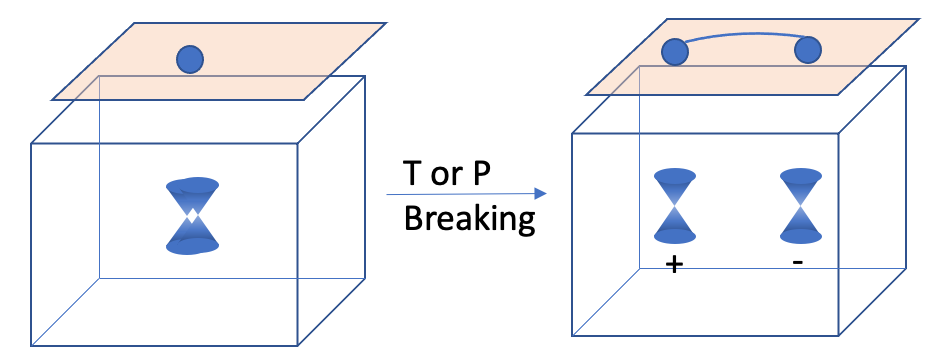
\includegraphics[width =\textwidth]{images/Weyl.png}
    \caption{ The Weyl semimetal, characterized by chiral gapless Weyl points within the bulk and a Fermi arc on the surface.
    On the left, an illustration depicts a fourfold degenerate Dirac point in the bulk, in the presence of time reversal symmetry ($T$) and inversion symmetry ($P$). 
    On the right, the creation of a Weyl semimetal through breaking either $T$ or $P$ is portrayed. This process results in two Weyl points of opposite chiralities being spatially separated in momentum space. The Weyl semimetal is protected by non-trivial Chern number and it host anomalous boundary states in the form of open Fermi arc.}
    \label{fig:Weyl}
\end{figure}

Taking the linear Weyl point  $H(\mathbf{k}) = \pm(\mathbf{k}-\mathbf{k^w})\cdot\mathbf{\sigma}$ with chirality $+$ or $-$,as an example, we can show the minium number of Weyl points that are required based on the $T$ and $P$ symmetries. These two symmetries operatss on the momentum and spins as follow:
\begin{equation}
\begin{aligned}
    T: \mathbf{k}\rightarrow-\mathbf{k}, \quad\mathbf{\sigma}\rightarrow-\mathbf{\sigma}\\
    P: \mathbf{k}\rightarrow-\mathbf{k}, \quad\mathbf{\sigma}\rightarrow\mathbf{\sigma}
\end{aligned}
\end{equation}
In the presence of time reversal symmetry, the $T$ operator maps a Weyl point at $\mathbf{k^w}$ to $-\mathbf{k^w}$, preserving the same chirality. As it is necessary for the total chirality to be zero, there must be another pair of Weyl points possessing the opposite chirality to the original Weyl points. Therefore, the minimum total number of Weyl points in a time-reversal symmetric system is four. On the other hand, under the inversion symmetry, there must be an additional Weyl point at $-\mathbf{k^w}$ with opposite chirality. Thus, the minimum total number of Weyl points in an inversion symmetric system is two. When both these symmetries coexist, each Weyl point has a time-reversal partner with the same chirality and an inversion partner with the opposite chirality, both at $-\mathbf{k^w}$. These points mutually annihilate and the band crossing is no longer topologically protected.


Like all topological phases that we discussed in the previous chapter, Weyl semimetal also exhibits the bulk-boundary correspondence priciple. Weyl semimetals host topological surface states  that originate from  a bulk topological invariant. However, unlike the surface states of a topological insulator, which have a Fermi surface composed of closed curves in momentum space, a Weyl semimetal hosts an exotic surface-state band structure that contains topological Fermi arcs, as shown in fig \ref{fig:Weyl}.


 \begin{figure}[h]
    \centering
    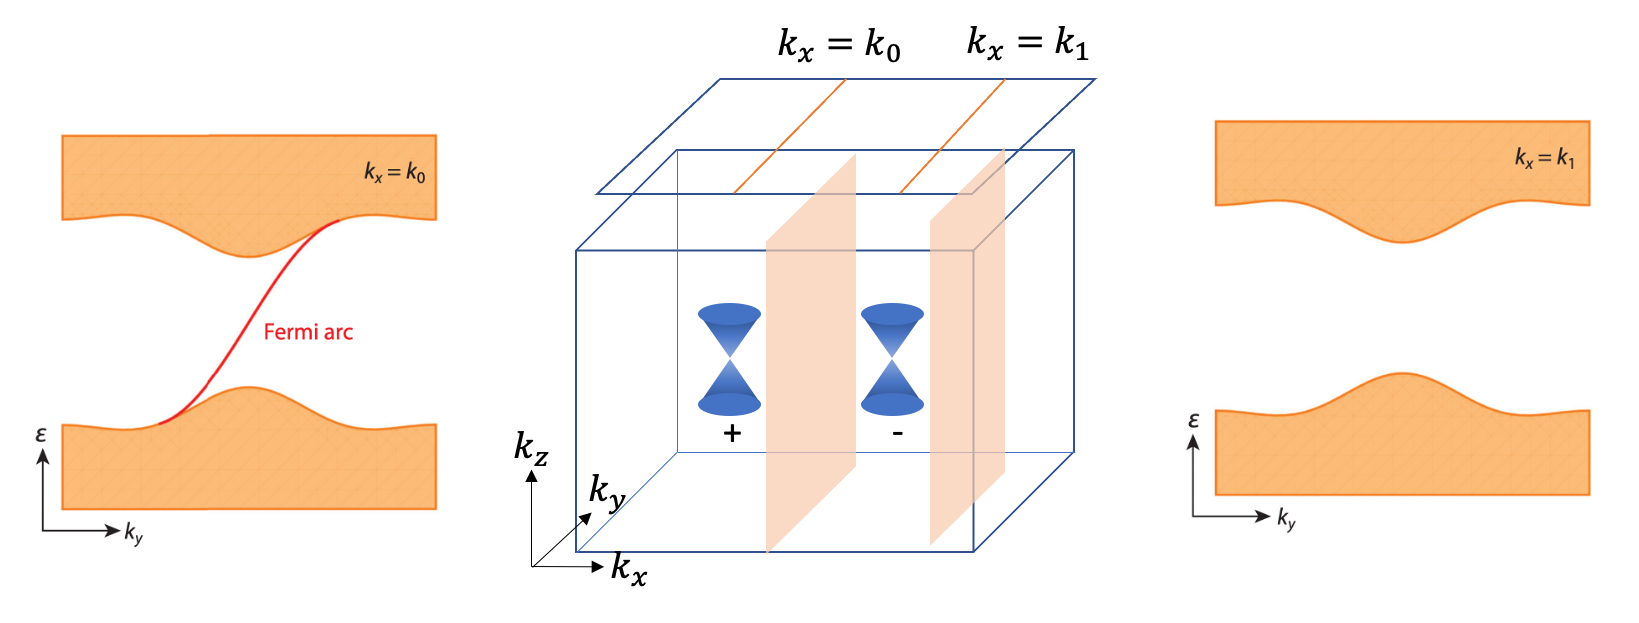
\includegraphics[width =\textwidth]{images/fermiarc.png}
    \caption{ An illustration of the formation of Fermi arc on the surface. Weyl points are separated along the $k_x$ direction. They are the srouce or sink of Berry flux. Weyl semimetal can be viewed as a set of two-dimensional slices which is perpendicular to the $k_x$ direction. On the left, for slices between the two Weyl points, a non-trivial Chern number is associated with the 2D system, and it hosts gapless chiral edge states. On the right, when the slices move beyond the Weyl points, the Chern number becomes trivial and no edge state is protected. The boundary stats of those sliced in the $k_xk_y$-plane  will stack along $k_x$ to form an open Fermi arc.
    }
    \label{fig:fermiarc}
\end{figure}
To illustrate this, consider a set of two-dimensional slices, with Weyl points separated along the $k_x$ direction as shown in fig \ref{fig:fermiarc}(middle). These slices are taken perpendicular to $k_x$. Any slice that does not contain Weyl points presents a gap, allowing the computation of a Chern number for that particular slice. As such, the three-dimensional band structure can be interpreted as a series of two-dimensional slices, each parameterized by $k_x$. As we move from $-k_x$ to $k_x$, the gap of the two-dimensional slice closes at the Weyl point, signifying a topological phase transition.

For slices between the two Weyl points, a non-trivial Chern number is associated with the 2D system, and it hosts gapless chiral edge states as shown in fig \ref{fig:fermiarc}(left and right). However, when the slices move beyond the Weyl points, the Chern number becomes trivial and no edge state is protected. The Weyl points can be perceived as the source and sink of the Berry flux. If we observe the boundary in the $k_xk_y$-plane, the set of chiral edge states will stack along $k_x$ to form anomalous surface states. These surface states, however, will terminate at the surface projections of the Weyl points, creating a Fermi arc on the surface. At the Fermi level, this Fermi arc will form an open curve on the surface.

The first material realization of Weyl semimetal is TaAs. It was theroretically predicted and experimental dicovered by Ding et al.\cite{weng2015weyl, lv2015experimental} Hasan et al.\cite{huang2015weyl, xu2015discovery, lee2015fermi} with ab initio calculation and ARPES. TaAs is an inversion breaking Weyl semimetal. Following its discovery, similar Weyl semimetal material like NbAs, NbP and TaP \cite{sun2015topological, lee2015fermi} were found. Weyl semimetals in magenetic materials, with time reversal breaking, have also been discovered in $ Co_3Sn_2S_2$\cite{liu2019magnetic}.Inheriting from their topological origins, Weyl semimetals display exotic transport properties, including negative magnetoresistance, non-local transport, chiral magnetic effect and chiral vortical effect. Those transport porperties have been demostrated through experiments and ab initial calculations in different materials\cite{wang2017quantum}.

The discovery of Weyl semimetals has significantly broadened our understanding of topological phases, particularly within gapless systems. More recently, the identification of increasingly exotic Weyl semimetal phases, such as Type-II Weyl semimetals\cite{soluyanov2015type, jiang2017signature, kumar2017extremely}, higher-order Weyl semimetals\cite{wang2020higher}, and non-Hermitian Weyl semimetals\cite{zyuzin2018flat}, has further expanded this field. Additionally, crystalline symmetries have considerably diversified the range of topological semimetals. Simultaneously, the existence of Kramers–Weyl fermions, a category of nodal fermions enforced by structural chirality, has also been found in  all non-magnetic chiral crystals with spin–orbit coupling\cite{chang2018topological}. $($TaSe$_4)_2$I has been recognized as a Type-III Weyl semimetal\cite{li2021correlated}, distinguished by two interconnected electron pockets as depicted in Figure \ref{fig:type3}.

 \begin{figure}[h]
    \centering
    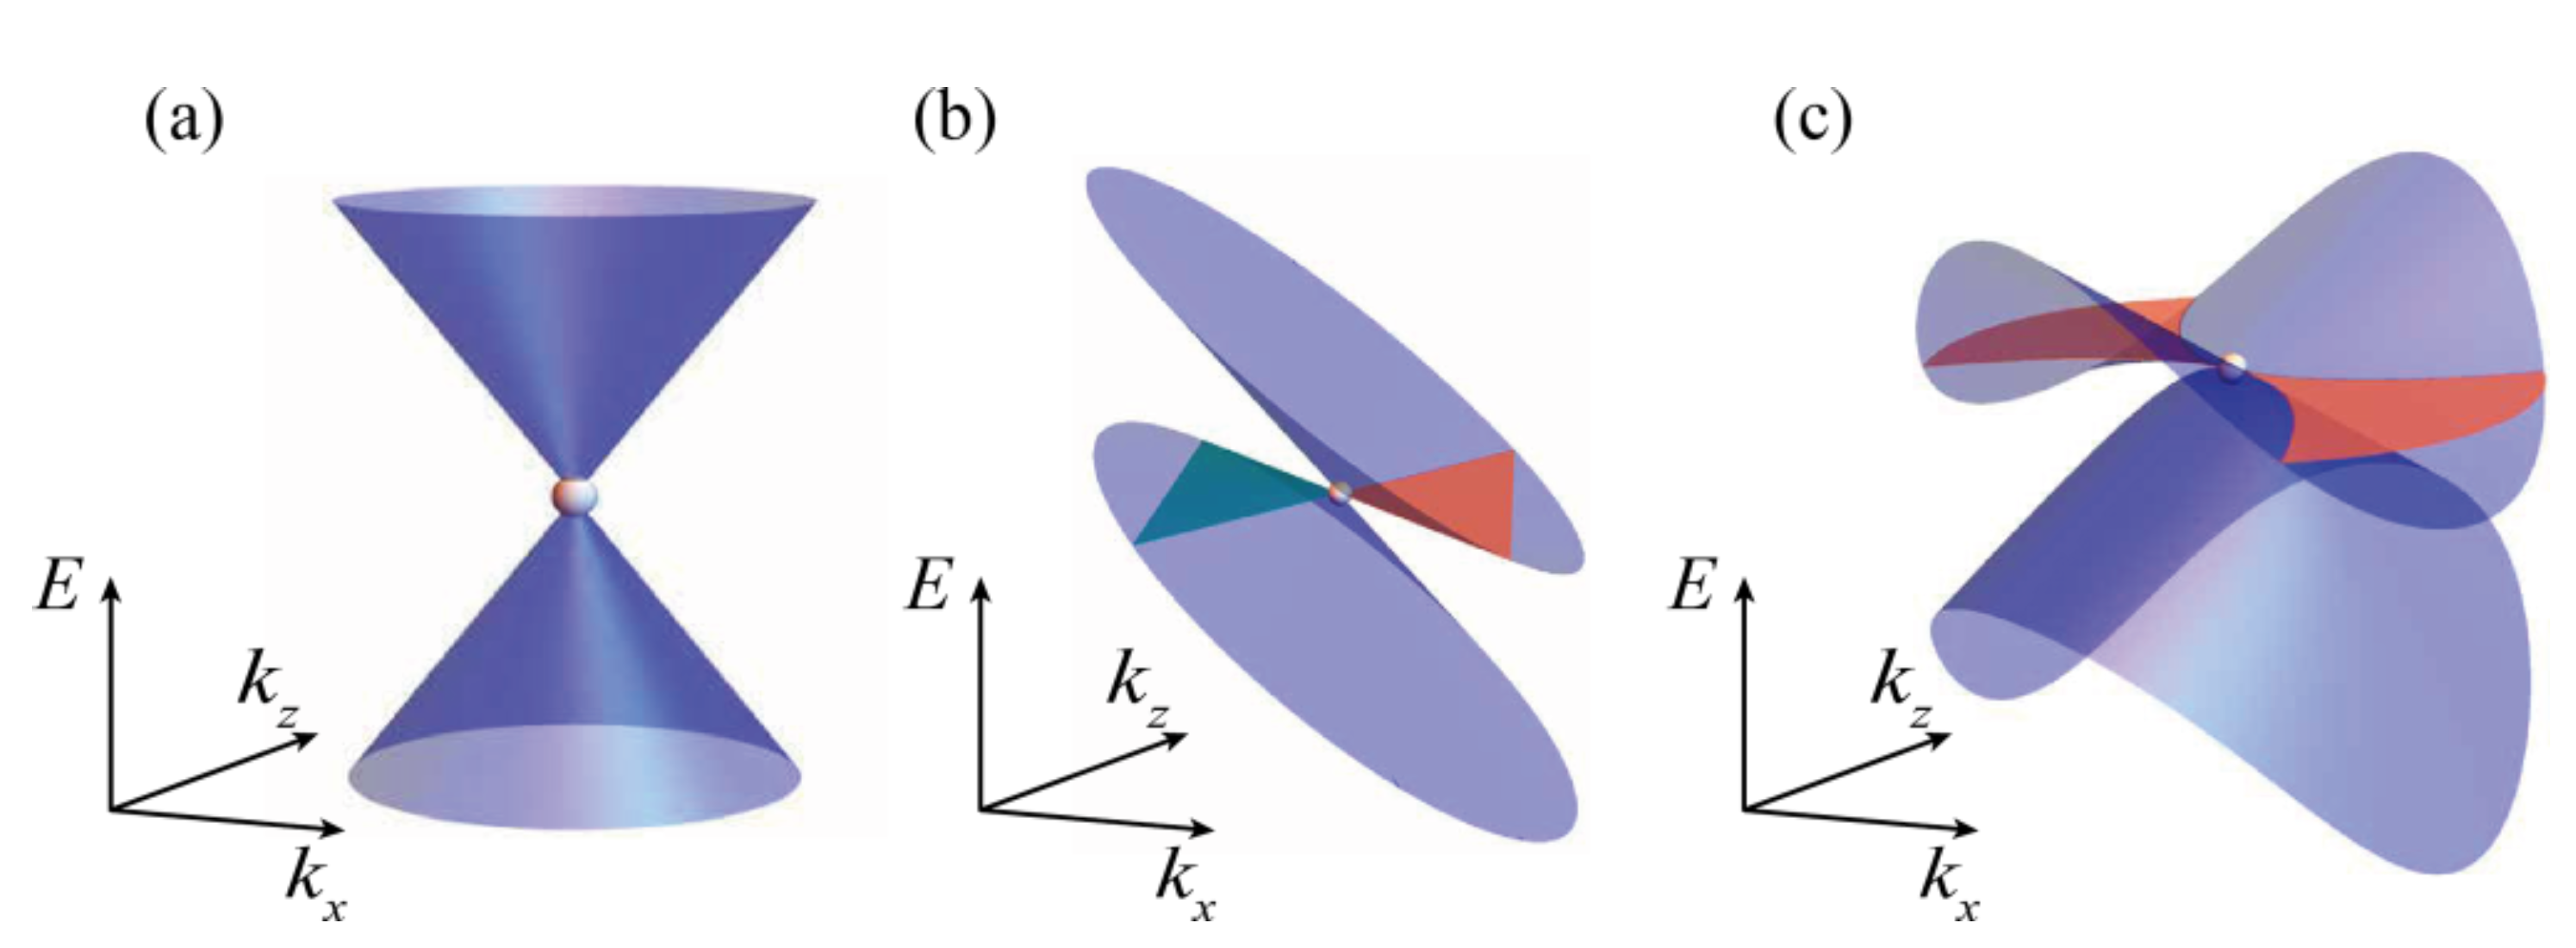
\includegraphics[width =\textwidth]{images/typeIII.png}
    \caption{ Xiao-Ping Li et al.\cite{li2021correlated} showed the representations of three distinct types of Weyl semimetals. (a) Type-I Weyl semimetal has pointlike electron and hole pockets. (b)Type-II Weyl semimetals has connected electron and hole pockets. Panel (c) portrays a type-III Weyl semimetal, characterized by two interconnected electron pockets (the analogous structure with two hole pockets corresponds to the case of an opposite quadratic tilting term).
    }
    \label{fig:type3}
\end{figure}

\section{Experimental features of $($TaSe$_4)_2$I}
\subsection{Crystal structure of $($TaSe$_4)_2$I}
Recently, there has been significant interest in understanding topological phenomena within quasi-1D materials. These materials, recognized as platforms for exploring topological physics since the pioneering work of Su, Schrieffer, and Heeger\cite{su1979solitons}, continue to provide valuable insights. Notable advancements include the identification of transitions between topological semimetals and charge density waves in $($TaSe$_4)_2$I\cite{shi2021charge,gooth2019axionic,sinchenko2022does,mu2021suppression,nenno2020axion,yi2021surface, zhang2020first}, as well as the discovery of superconductivity within topological semimetals in $($NbSe$_4)_2$I\cite{pei2021pressure}. Both these findings stem from the family of halogen transition-metal tetrachalcogens $($MX$_4)_x$Y\cite{van2001structure} compounds, where M represents Ta or Nb, X stands for S, Se, or Te, Y indicates I, Br, or Cl, and $x$ is greater than or equal to 2. Further intriguing findings involve potential transitions between Weyl semimetals and charge density waves in Y$_2$Ir$_2$O$_7$, which originate from correlated pyrochlore iridates, R$_2$Ir$_2$O$_7$ (R = Y, Eu, Nd)\cite{juyal2022possible}
In addition, the exploration of magnetism's interaction with topology in Sm$_3$ZrBi$_5$\cite{khoury2022class}, part of the Ln$_3$MPn$_5$ compound family (where Ln ranges from La to Nd, M includes Ti, Zr, Hf, Mg, Mn, and Nb, and Pn is either Bi or Sb), has also deepened our understanding of these phenomena. 


The focus of this thesis is the theoretical exploration of topological physics, inspired by the transition between Weyl semimetal and charge density wave in $($TaSe$_4)_2$I. First synthesized by P. Gressier, L. Guemas, and A. Meerschaut in 1982\cite{gressier1982preparation}, $($TaSe$_4)_2$I is a quasi-one-dimensional, non-magnetic material that has long served as a study model for the intricate multi-domain CDW phases\cite{van2001structure}.

$($TaSe$_4)_2$I is a member of the $($MX$_4)_x$Y compound family. In these compounds, columns of MX$_4$ are arranged in a 2D lattice, interspersed with chains of halogenide atoms. At room temperature, $($TaSe$_4)_2$I crystallizes into a body-centered tetragonal structure in space group $97(I422)$, with lattice parameters $a_0 = b_0= 9.531$ Å and $c_0= 12.824$ Å.

As depicted in Fig \ref{fig:crystal_structure}(a) and (b), the conventional unit cell of $($TaSe$_4)_2$I consists of two TaSe$_4$ chains running parallel to the c-axis, separated by four iodine atoms. Each chain comprises four alternating layers of Ta atoms and rectangles, with four Se atoms located at each corner as illustrated in Fig \ref{fig:single_chain}. This arrangement yields a total of 4 Ta atoms and 16 Se atoms per chain, leading to the chemical formula $($TaSe$_4)_8$I$_4$ for each conventional unit cell, as seen in Fig \ref{fig:crystal_structure}. Given the body-centered lattice structure of the material, its primitive unit cell contains half the number of atoms present in the conventional cell.

\begin{figure}[h]
    \centering
    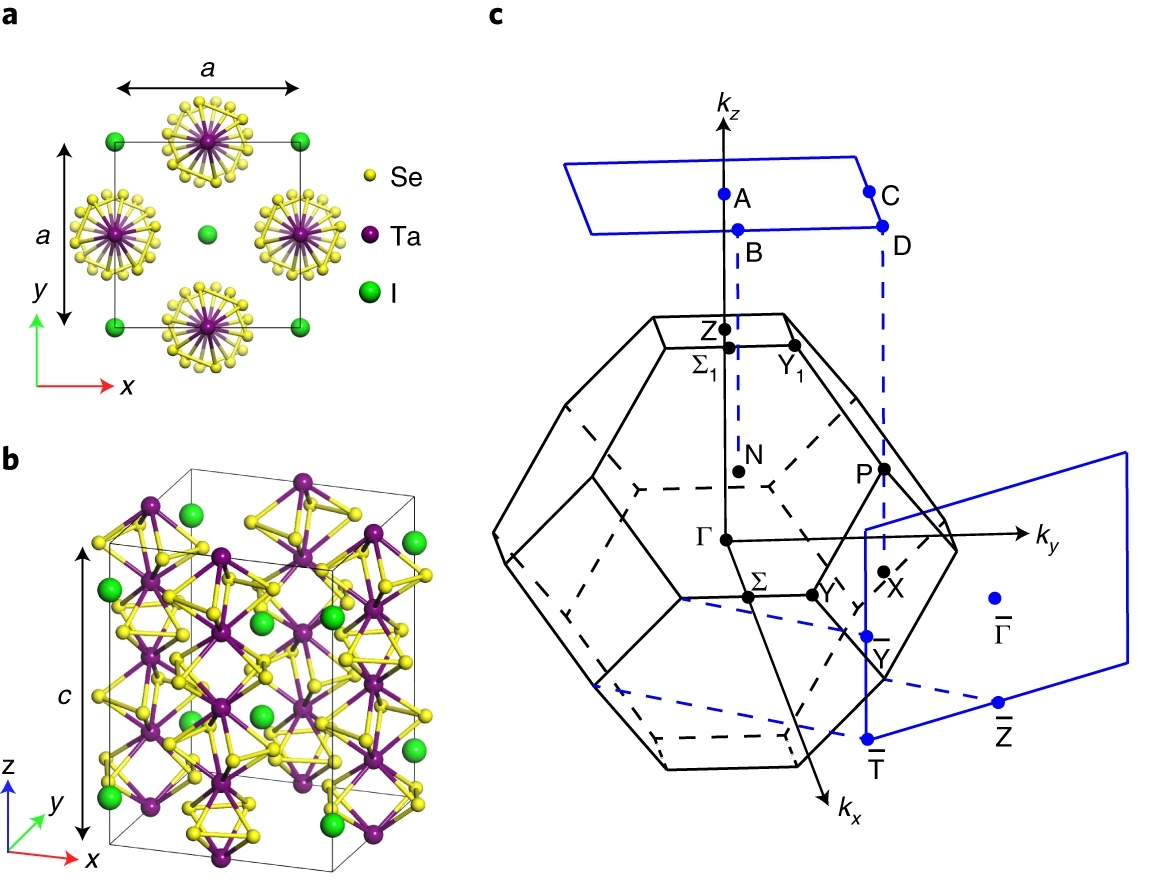
\includegraphics[width =\textwidth]{images/crystal_structure.jpg}
    \caption{Crystal structure, 3D bulk and 2D surface Brillouin zones of $($TaSe$_4)_2$I.\cite{shi2021charge}  (a)The conventional unit cell viewing from the top (001), the TaSe$_4$ chains are arranged in two-dimentional checkerboard lattice. The lattice constant along $x$ and $y$ direction are the same $a_0 = b_0= 9.531$ Å. (b) The conventional unit cell viewing from the side.$($TaSe$_4)_2$I is a quasi-one-dimensional crystal in  space group 97 ($I422$). (c) The Briullium zone of the $($TaSe$_4)_2$I lattice which is in body-centered tetragonal structure. $($TaSe$_4)_2$I is symmorphic and non-magenetic with body-centered lattice translations, four-fold roation along $z$-axis $C_{4z}$, two-fold rotaion along $x$-axis $C_{2x}$ and time reversal symmetry $T$.}
    \label{fig:crystal_structure}
\end{figure}

\begin{figure}[h]
    \centering
    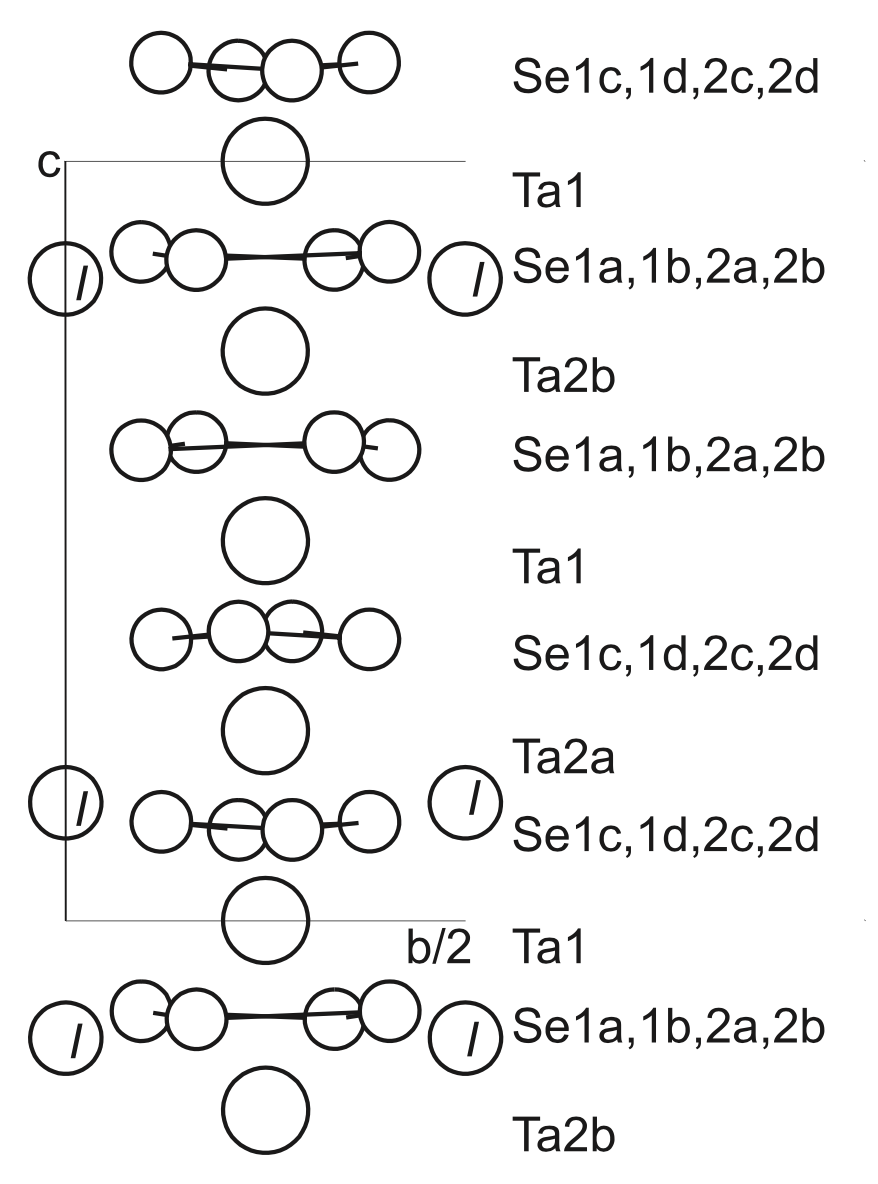
\includegraphics[width =0.5\textwidth]{images/signlechain.png}
    \caption{Crystal structure of an isolated $($TaSe$_4)$ chain in $($TaSe$_4)_2$I viewing from the side. Each chain comprises four alternating layers of Ta atoms and rectangles with four Se atoms located at each corner. The chain exhibits nonsymmorphic screw symmetries.  Chains are separated by four iodine atoms.\cite{van2001structure}}
    \label{fig:single_chain}
\end{figure}

Viewing from the top (001) as shown in Fig \ref{fig:crystal_structure}(a), the TaSe$_4$ chains are arranged in two-dimentional checkerboard lattice. When isolated shown in Fig \ref{fig:single_chain}, each TaSe$_4$ chain exhibits nonsymmorphic screw symmetries, because of the stacking order of selenium rectangles. However, the crystalline symmetries of $($TaSe$_4)_2$I are symmorphic and contain the body-centered lattice translations, four-fold roation along $z$-axis $C_{4z}$ and two-fold rotaion along $x$-axis $C_{2x}$. It is also structurally chiral and have strong spin orbital coupling(SOC).
Additionally, $($TaSe$_4)_2$I respects time-reversal symmetry (TRS) because it is nonmagnetic.



\subsection{The phases in high and low temperatures}
The quasi-one-dimensional $($TaSe$_4)_2$I undergoes a Peierls transition, as discussed in Chapter \ref{ch:cdw1d}. The critical temperature for this transition is reported to be around $T_c=263$K \cite{gooth2019axionic} or $T_c=248$K \cite{shi2021charge}, with the exact value varying depending on the specific samples under study. As depicted in Fig \ref{fig:phasetransition}, the peak of derivative in electrical resistivity measurements demonstrate a phase transition from a metallic to an insulating state as the temperature decreases from room temperature \cite{gooth2019axionic}. Furthermore, recent Angle-Resolved Photoemission Spectroscopy (ARPES) experiments \cite{shi2021charge}, as shown in Fig.\ref{fig:ARPAS}, reveal significant changes in the band gap size across different temperature phases. In the low-temperature phase, the band gap is approximately 0.12 eV. However, in the high-temperature phase, the band gap significantly reduces to 0.04 eV. This alteration in the band gap size signifies a phase transition from a Charge Density Wave (CDW) state to a Weyl semimetal state.

\begin{figure}[h]
    \centering
    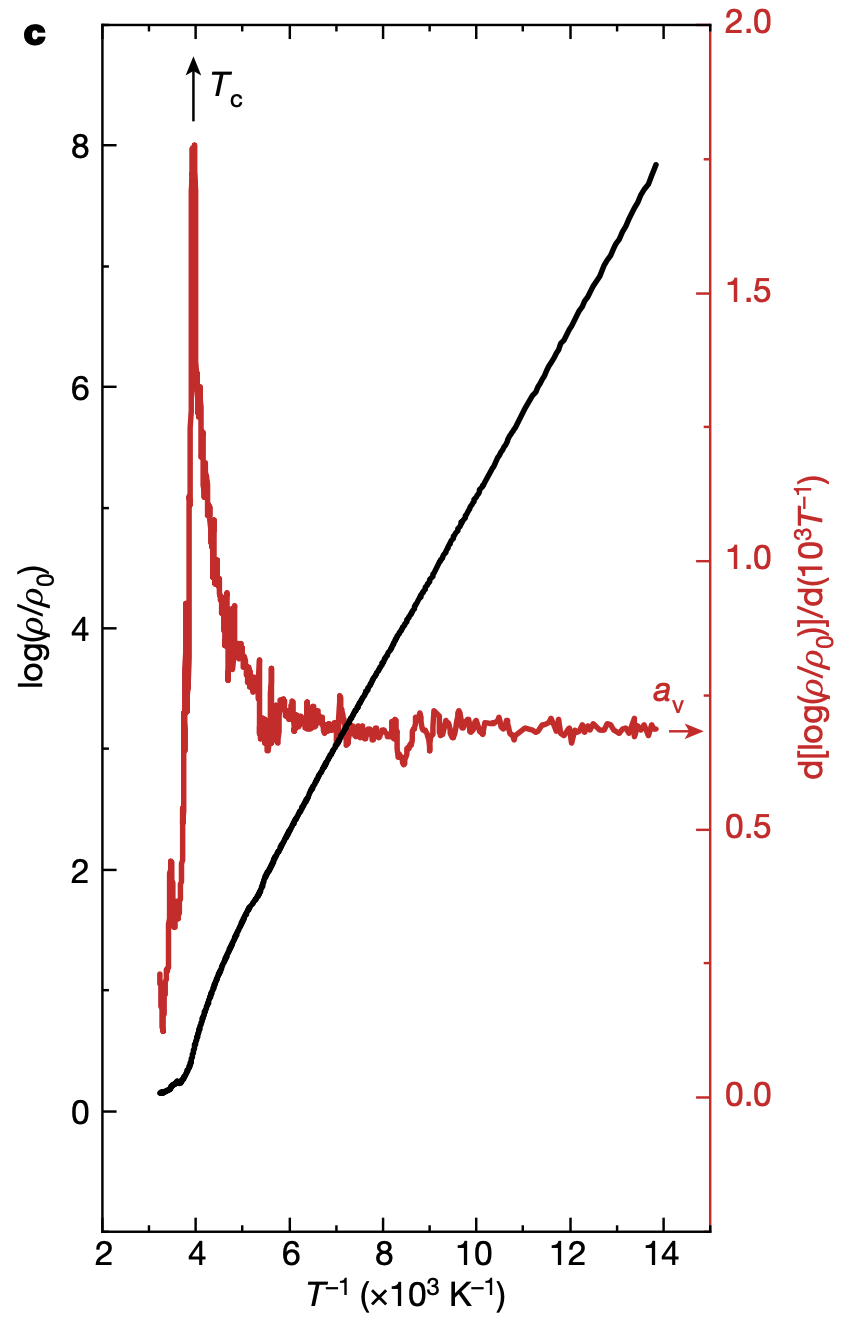
\includegraphics[width =0.5\textwidth]{images/phasetransition.png}
    \caption{The measurement of electrical resistivity as a function of temperature for $($TaSe$_4)_2$I. The raw data is represented by the black line, while the derivative is shown by the red line. A distinct peak is observed at the critical temperature, approximately $T_c=263K$. This peak signifies a phase transition from a metallic to an insulating state as the temperature decreases from room temperature \cite{gooth2019axionic}.}
    \label{fig:phasetransition}
\end{figure}

In its high-temperature phase, $($TaSe$_4)_2$I was previously classified as a metal with a linear crossing near the Fermi energy ($E_f$). Recent first-principle calculations and experiments have demonstrated that $($TaSe$_4)_2$I is a Weyl semimetal when the temperature exceeds $T_c$. In this Weyl semimetal phase, two types of Weyl fermions exist in the bulk.

A total of 48 Weyl fermions, referred to as Fermi surface Weyl points (FSWPs), are situated close to the Fermi energy, specifically within the vicinity of 15 meV to $E_f$. These 48 FSWPs are distributed near the plane $k_z=\pm\frac{\pi}{c}$, shown in Fig \ref{fig:FSWPs}. Furthermore, due to the chiral structure of $($TaSe$_4)2$I and strong spin-orbit coupling (SOC), the $C_{4z}$ symmetry enforces 8 Kramers-Weyl points along the $k_z$-axis resident between 16 to 20 mev below $E_f$ \cite{chang2018topological}.

The Chern numbers of chiral fermions (Weyl fermions), which represent monopole chiral charges, remain invariant under symmorphic rotations and time-reversal operation (T). Consequently, Weyl points with opposite chirality can exist at different energies within $($TaSe$_4)_2$I. This energy offset between oppositely charged chiral fermions was previously only predicted in Kramers-Weyl and unconventional fermion semimetals. $($TaSe$_4)_2$I represents a rare example of a conventional Weyl semimetal exhibiting an energy offset.

As discussed in the previous section \ref{sec:weyl}, Weyl semimetals harbor topological Fermi-arc surface states, which contribute to unconventional transport properties. In $($TaSe$_4)_2$I, first principle calculations reveal the existence of Fermi-arcs bridging islands of bulk state projections on the (110), (100), and (011) surfaces. Figure \ref{fig:weyl_points}(b) illustrates the surface states of $($TaSe$_4)_2$I when terminated in the experimentally favored (001) direction, thereby capturing its topological properties.
The projected Fermi pockets indicate a Chern number equal to 8 at the corner and center of the surface Brillouin zone. The eight Kramers-Weyl points are primarily clustered along the $k_z$-axis, with very minimal separation in the $k_xk_y$-plane, and carry zero net chiral charge. Thus, their contribution to the Fermi-arc surface state is effectively negligible.

\begin{figure}[h]
    \centering
    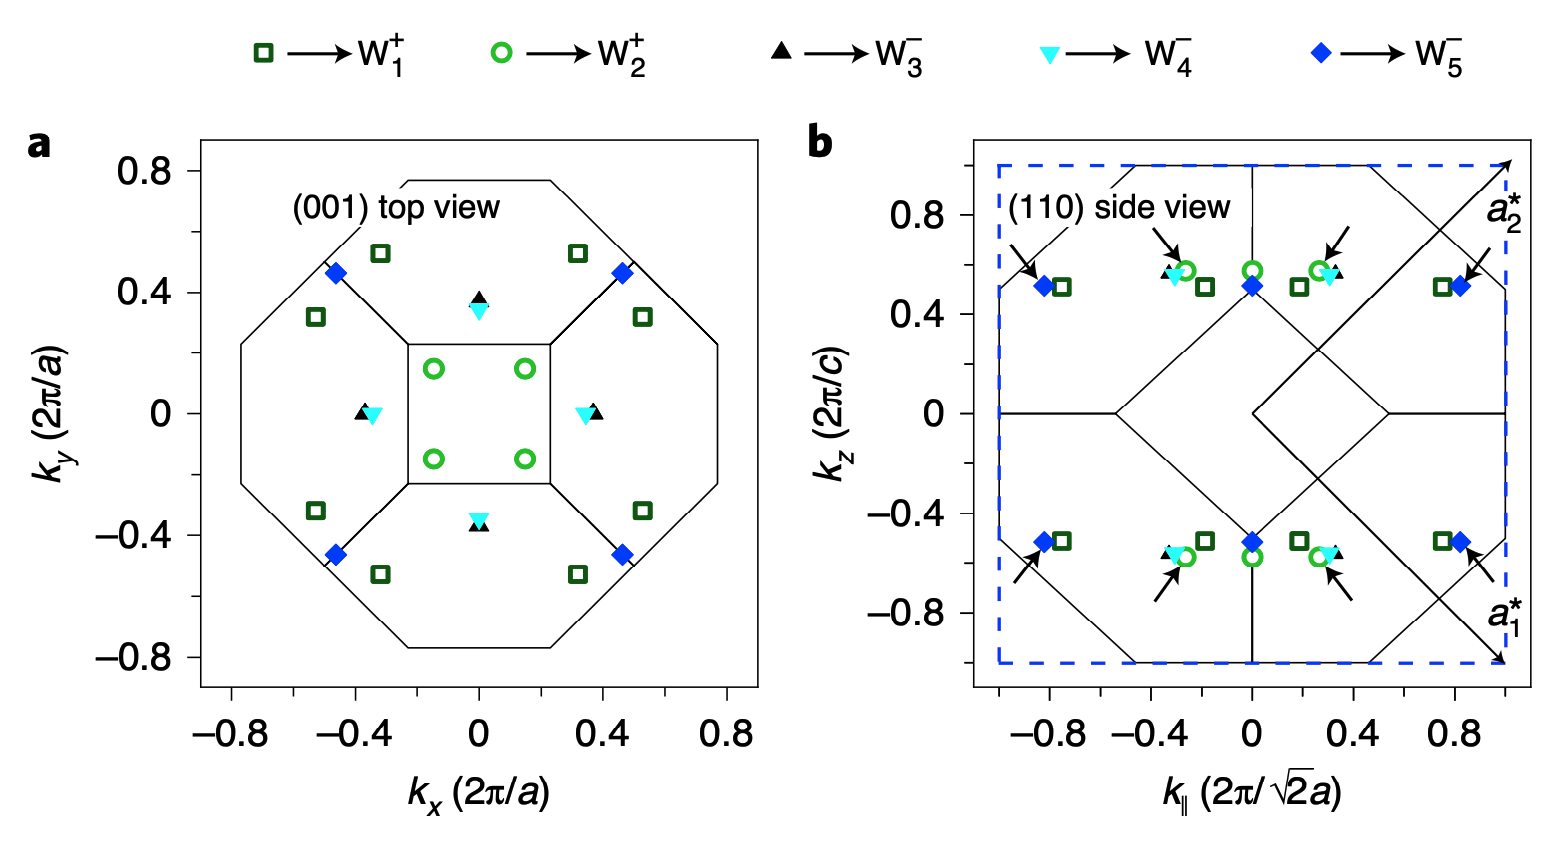
\includegraphics[width =\textwidth]{images/FSWPs.png}
    \caption{The first priciple calculation showing the position of 48 Weyl fermions at Fermi surface. They are distributed near the plane $k_z=\pm\frac{\pi}{c}$. \cite{shi2021charge}}
    \label{fig:FSWPs}
\end{figure}

$($TaSe$_4)_2$I is known to transition into an incommensurate gapped CDW phase when cooled just below room temperature, a phenomenon that has been studied for over three decades \cite{gressier1982preparation,tournier2013electronic}. Electrical resistivity measurements confirm the CDW's critical temperature and a band gap of approximately 260 meV. In the absence of a magnetic field, the material exhibits linear Ohmic behavior when a direct current is applied, both at low and high temperatures. The resistance remains constant with increasing temperature in the high-temperature phase. However, below the critical temperature $T_c$, the resistance of $($TaSe$_4)2$I begins to decrease once the applied voltage surpasses a certain threshold, denoted as $V_{th}$. This voltage threshold is indicative of the pinning potential generated by impurities, which impedes the motion of CDWs.



\subsection{Recent debates on $($TaSe$_4)_2$I}
Weyl semimetals serve as the foundation for a broad range of topological phases in three dimensions. The introduction of various types of coupling or interaction can transition a Weyl semimetal into different topological phases. For instance, the introduction of a spatial or charge U(1) symmetry-breaking single-body mass can transform it into a topological insulator or superconductor. Moreover, the introduction of symmetry-preserving many-body gapping interactions can lead to an insulating topological phase that carries long-range entanglement and non-trivial topological order \cite{raza2019dirac}. In the context of the phase transition from a Weyl semimetal to a charge density wave  in $($TaSe$_4)_2$I, there has been debate surrounding the topology of its CDW phase. Specifically, questions have arisen regarding whether the gapped CDW phase is an axion insulator.

Axion insulators are a class of topological materials that have attracted significant interest in the field of condensed matter physics due to their unique properties and potential applications. These insulators are named after the hypothetical axion particle from particle physics and are distinguished by a unique electromagnetic field response, which can be described by an axion term in the electromagnetic action\cite{peccei1977cp, wilczek1987two,svrcek2006axions}. The axion coupling, denoted as $\theta$ in 3D, is analogous to the Berry phase 
$\phi$ in 1D. 
Starting from the integration of the first Chern number in 2D, as discussed in Equation \ref{eq:chern}, the Berry phase can be expressed through a dimension reduction as:

\begin{equation}
\phi=\int_{B Z} d k \operatorname{Tr}[\mathcal{A}]
\end{equation}

In physics, this equation describes the polarization in one dimension:
\begin{equation}
P=-e\frac{\phi}{2\pi}.
\end{equation}

A similar procedure can be applied starting from the integration of the second Chern number, which is defined in four dimensions. After integrating over one dimension with dimension reduction, the Chern-Simons axion coupling term can be written as:

\begin{equation}
\theta=-\frac{1}{4 \pi} \int_{B Z} d^3 k \epsilon^{\alpha \beta \gamma} \operatorname{Tr}\left[\mathcal{A}_\alpha \partial_\beta \mathcal{A}_\gamma-i \frac{2}{3} \mathcal{A}_\alpha \mathcal{A}_\beta \mathcal{A}_\gamma\right].
\end{equation}
Similar to 1D case, gauge transformation
\begin{equation}
A_\mu \longrightarrow U^{\dagger} A_\mu U+i U^{\dagger} \partial_\mu U
\end{equation}
shifts $\theta$ by $2\pi$, $\theta\rightarrow\theta+2n\pi, n\in\mathbb{Z}$, so the axion coupling is only well defined modulo $2\pi$. This term in physics gives the magentoelectric tensor:
\begin{equation}
    \alpha=\frac{e^2}{h}\frac{\theta}{2\pi}
\end{equation}
with an axionic effective action $\theta$ therm coupling the electric and magnetic field in the same direction,
\begin{equation}
    S_\theta=\frac{e^2}{4\pi^2}\int dt dr\quad \theta\mathbf{E}\cdot\mathbf{B}
\end{equation}
This implies that an electric field will induce a parallel magnetization proportional to  $\alpha$. The axion term leads to an extension of Maxwell-equation in the material: 

\begin{equation}
\begin{aligned}
\nabla \cdot \mathbf{E}= & 4 \pi \rho-\frac{\alpha}{\pi}(\nabla \theta) \cdot \mathbf{B} \\
\nabla \times \mathbf{B}= & \frac{4 \pi}{c} \mu_0 \mathrm{~J}+\frac{1}{c} \frac{\partial \mathrm{E}}{\partial t}  \\& +\frac{\alpha}{\pi}\left[\frac{1}{c} \mathbf{B}\left(\frac{\partial}{\partial t} \theta\right)+(\nabla \theta) \times \mathrm{E}\right]
\end{aligned}
\end{equation}
where $\theta$ serves as a dynamic axion field. The low energy contribution to this value is dictated by the nuanced topological characteristics of the band structure in the condensed matter system. It's important to note that an observable effect is only shown when there's a change in $\theta$ over space or time.\cite{nenno2020axion}


Dynamical axion fields exhibit a unique magnetoelectric effect, where an applied electric field can induce a magnetic polarization, and conversely, a magnetic field can induce an electric polarization. The manifestation of axion electrodynamics in Weyl semimetals is a result of the spatial and energy separation of band crossings, or Weyl nodes, with contrasting chirality.\cite{wang2013chiral} In certain material systems, when a Weyl semimetal transitions to a charge density wave phase, it opens up a gap in the energy bands. The resulting gapped phase is predicted to be an axion insulator.\cite{wang2013chiral, wei2012excitonic,laubach2016density,you2016response}

Experimentally, the magnetoelectric transport can be measured by applying a magnetic field parallel to the electric field, which results in the phason current contributing to the transport. Recent studies on $($TaSe$_4)_2$I have demonstrated this by measuring the change in non-Ohmic behavior in its low-temperature charge density wave phase. As shown in Fig \ref{fig:megnetoelectric}, at $T=80K$, below the critical temperature $T_c$, the $V-I$ plot shows a strong correlation with the magnitude of the parallel magnetic field when exceeding the voltage threshold $V_{th}$. As the magnitude of $B$ or $E$ increases, the experiment shows an enhancement in the magnetoconductance, aligning with the phason current from the dynamic axion field. Conversely, because $\theta$ only couples with the $\mathbf{B}\cdot\mathbf{E}$ term, any magnetic field perpendicular to the electric field will not contribute to the transport, which is also consistent with experimental observations\cite{gooth2019axionic}. However, whether the measurements in this experiment are sufficient to demostrate the signatures of axion electrodynamics in CDW state, given that the transport signature only appears at $80K$, is currently a topic of intense debates.\cite{sinchenko2022does}

\begin{figure}[h]
    \centering
    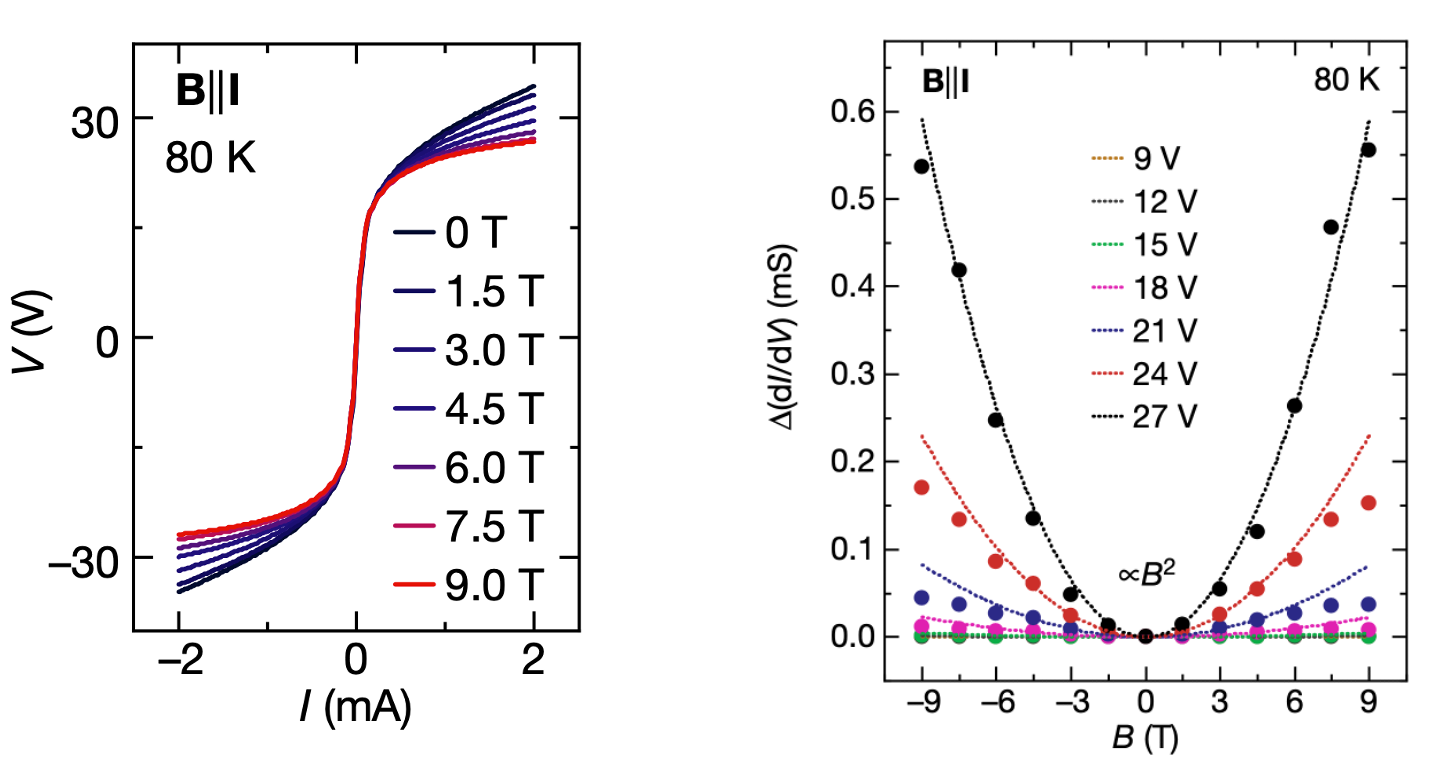
\includegraphics[width =\textwidth]{images/phason.png}
    \caption{Magnetoelectric transport experimental results for $($TaSe$_4)2$I in the charge density wave phase. The magnetic field is applied parallel to the electric field. At $T=80K$, which is below the critical temperature $T_c$, the $V-I$ plot (depicted on the left) exhibits a strong correlation with the magnitude of the parallel magnetic field when surpassing the voltage threshold $V{th}$. As the magnitude of $B$ or $E$ escalates, the experiment reveals an enhancement in the magnetoconductance (illustrated on the right), consistent with the phason current from the dynamic axion field. \cite{shi2021charge}}
    \label{fig:megnetoelectric}
\end{figure}



By imposing symmetry constraints, the axion term 
$\theta$ can assume quantized values. In fact, any crystalline symmetry that preserves pseudoscalar forces 
$\theta$ to take only two values, 
\begin{equation}
\theta= \begin{cases}0 & \text { (topologically trivial) } \\ \pi & \text { (topologically nontrivial) }\end{cases}
\end{equation}
leading to a $\mathbb{Z}_2$ topological classification. For $\theta=\pi$, the system is topologically non-trivial. There are many symmetries that can preserve pseudoscalar, such as time reversal symmetry, inversion symmetry, or any other operator that would reverse the sign of a pseudoscalar\cite{vanderbilt2018berry}. In the case where only time reversal symmetry is present, as is the case for strong topological insulators, the classification aligns with $\mathbb{Z}_2$. When $\theta=\pi$ is protected by any symmetry other than time reversal symmetry, we refer to it as an axion insulator.

The smoking gun experimental evidence of the axion charge density wave phase is the presence of axion strings. These are one-dimensional in-gap topological modes tied to the defects of the charge density wave (CDW). Recent experiments have reported varying results, with some noting the presence\cite{litskevich2022observation} and others the absence\cite{huang2021absence} of axion strings, contingent on the specifics of the experiment and the sample. Further studies are necessary to conclusively determine whether $($TaSe$_4)_2$I is an axion insulator.

\begin{figure}[h]
    \centering
    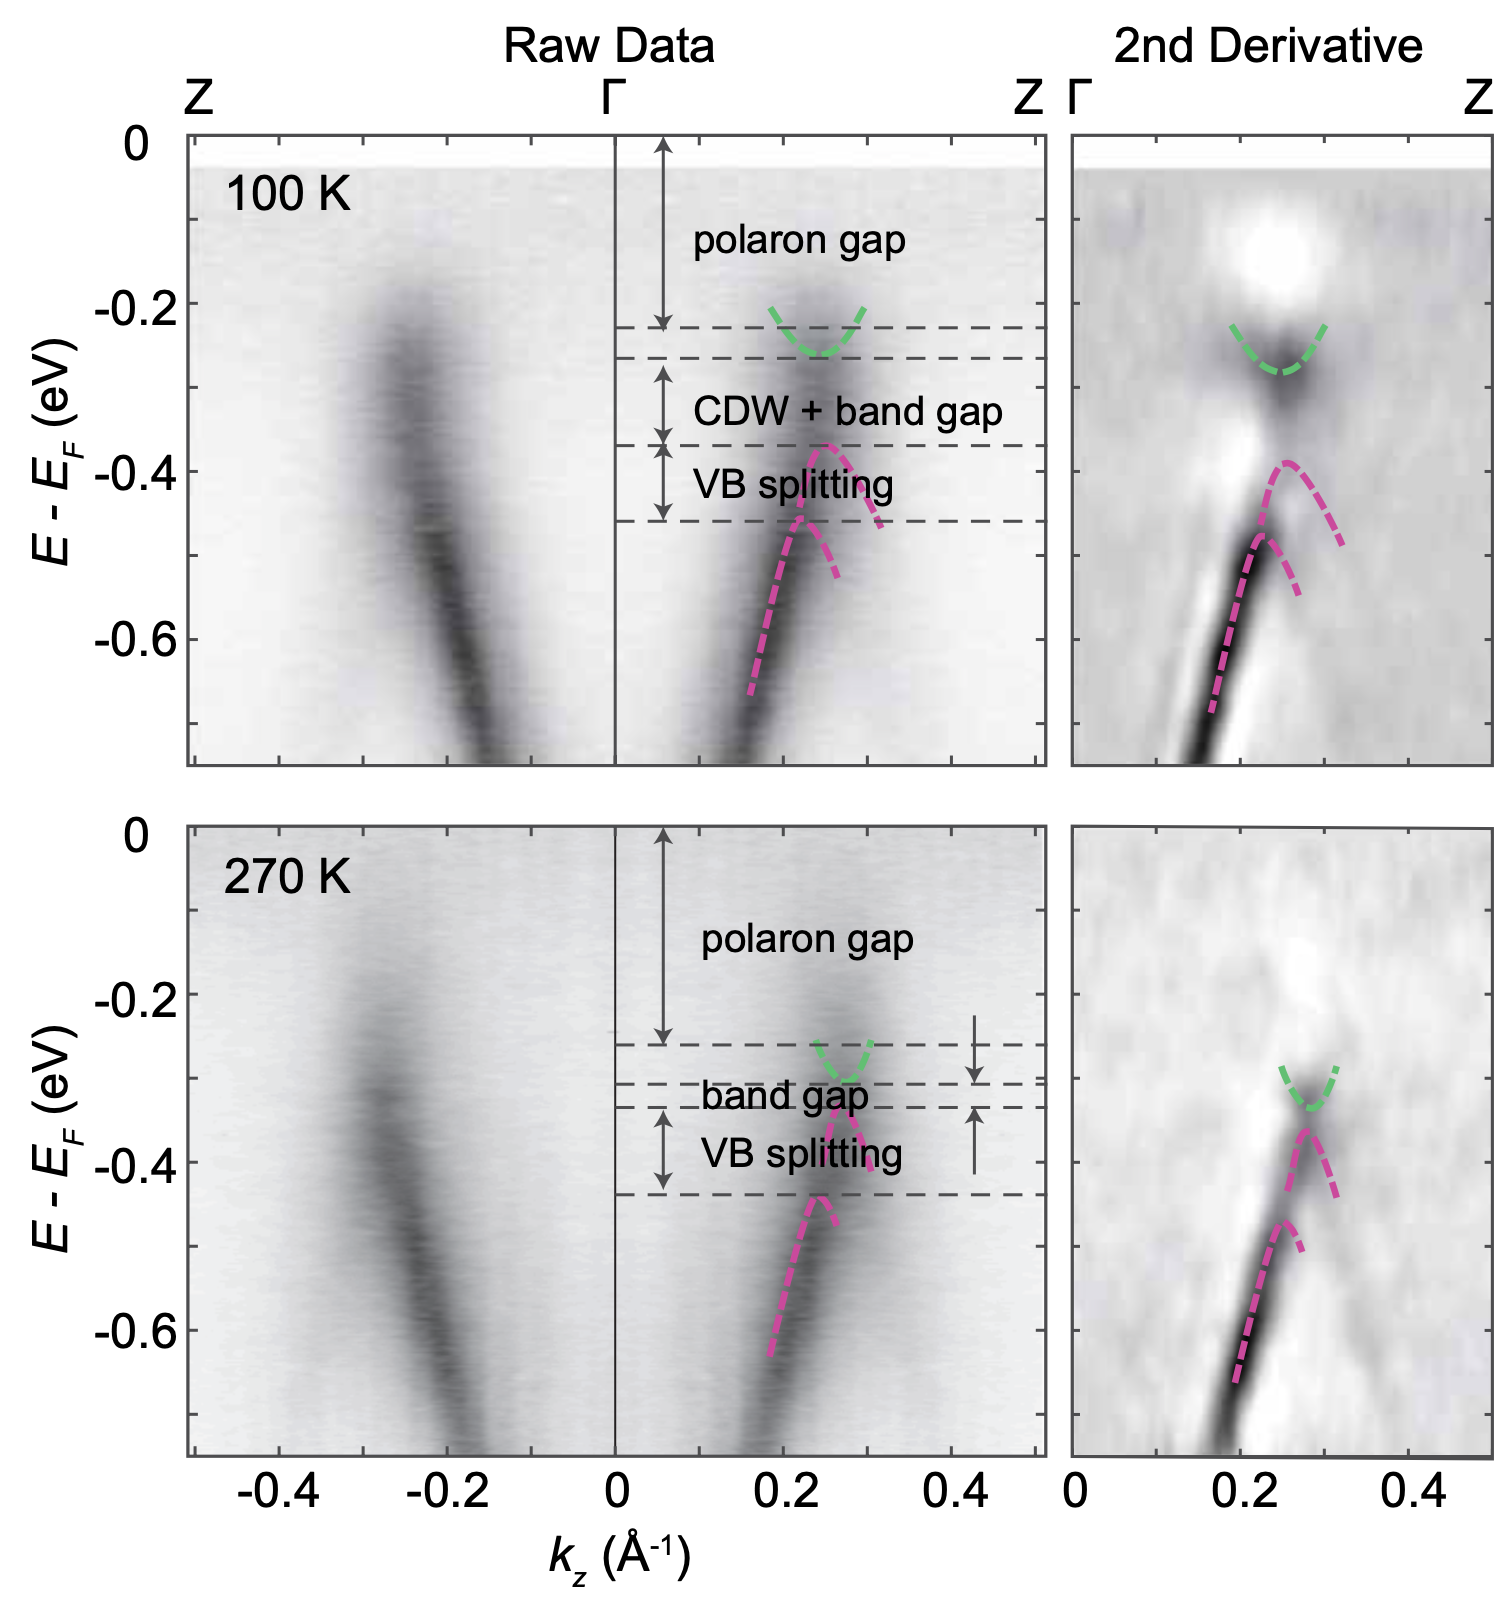
\includegraphics[width =\textwidth]{images/ARPAS.png}
    \caption{The results from Angle-Resolved Photoemission Spectroscopy (ARPES) experiments conducted on $($TaSe$_4)_2$I are presented for both low-temperature (upper) and high-temperature (lower) phases. The left plots depict the energy dispersion along the $\Gamma$-$Z$ direction, while the right plots represent the second derivative of the raw data. The valence and conduction bands are delineated by dashed magenta and green lines, respectively. In the low-temperature phase, the band gap is approximately 0.12 eV. However, in the high-temperature phase, the band gap significantly reduces to 0.04 eV. This change in the band gap size indicates a phase transition from a Charge Density Wave (CDW) state to a Weyl semimetal state. \cite{shi2021charge}}
    \label{fig:ARPAS}
\end{figure}

%\section{Experiment features of $($TaSe$_4)_2$ I}